\documentclass[a4paper]{article}

\usepackage[natbib=true,style=authoryear-comp,backend=biber,doi=false,url=false,isbn=false]{biblatex}
\bibliography{paper}

\usepackage{todonotes}
\usepackage{a4wide}
\usepackage{amsmath}
\usepackage{amssymb}
\usepackage{syllogism}
\usepackage{subcaption}


\usepackage{xcolor}
\definecolor{Red}{RGB}{178,34,34}
\newcommand{\mf}[1]{\textcolor{Red}{[mf: #1]}}

\begin{document}

\title{Natural sources of vagueness and their implications}
\author{Jos\'e Pedro Correia \and Michael Franke}
\date{}

\maketitle

\begin{abstract}
A vexing puzzle about vagueness, rationality and evolution runs, in crude abbreviation, as follows: vague language use is demonstrably suboptimal if the goal is efficient precise and cooperative information transmission; hence rational deliberation or evolutionary selection should, under this assumed goal, eradicate vagueness from language use.
Since vagueness is persistent in all human languages, something has to give.
In this paper, we investigate a number of reasons why and mechanisms how vagueness may come into the picture in formal models of rational or evolutionary optimal signaling.
We show how uncertainty about not only the linguistic practices of others, but also about the world itself can lead to vagueness, and how, given vagueness, natural linguistic practices are likely to create more reason for vagueness.
We explore the consequences of these reasons and mechanism for a notion of meaning and a notion of language.
\end{abstract}

\tableofcontents

\section{Vagueness}
\label{sec:vagueness}

The classic philosophical problem of vagueness is most starkly embodied by the sorites paradox.
The original formulation is attributed to Eubulides, an ancient Megarian philosopher~\parencite{sorensen_sorites_2009}, and uses the example of a heap of sand: if no removal of one grain of sand can make a heap into a non-heap, we can repeatedly remove all but one grain of sand of something that is clearly a heap and be forced to acknowledge that the remaining single grain of sand is still a heap; otherwise, it seems, we would have to accept that there is a determinate number of grains that forms a heap, and anything under it is not a heap.
Neither choice is, however, intuitively satisfying.
The paradox is interesting because it can be made general and re-applied to many other words besides `heap'.
Predicates for which one can find a suitable instance of the general formulation of the sorites paradox are called \emph{vague}.
Paradigmatic examples besides `heap' include `tall', `red', `bald', `tadpole', and `child'~\parencite{Keefe1997}.
How widespread is the problem?
It is easy to find more examples of predicates based on more finely grained properties---as `tall' is intuitively based on height---for which constructing a sorites paradox would be easy.
Mereological nihilists argue that instances of the sorites can be designed for any material object that can be decomposed into small enough parts.
If we subscribe to the scientific picture of matter as composed of molecules and atoms, this applies to tables and chairs, cats and mats, and any other ordinary thing~\parencite{Unger1979}.
Bertrand Russell famously argued~\parencite*{russell_vagueness_1923} that all words, including ``the words of pure logic'', are vague when used by human beings.
The problem thus seems to be a serious one.
But it does not obviously undermine our everyday practices, so the issue must be with the conceptions we have of the mechanisms that underlie them.

Vagueness is typically seen as a challenge to the classical conception of language and meaning.
One problem is that vague predicates seem to lack precise boundaries; if that is the case, how can words like `tall' stand in correspondence to something like a well defined set of tall people?
And if we cannot know exactly whether a certain person is `tall' or not, as with borderline cases, how are we to determine the truth value of sentences that involve statements of tallness regarding these borderline cases?
Supervaluationism, many-valued logics, and degree theories all propose changes to the classical picture in order to accommodate for vague predicates.
They are, however, still strongly committed to retaining as much as possible of it, particularly the core notions of truth and reference.
Mark Sainsbury~\parencite*{sainsbury_concepts_1999} argues that, because of that, they all fail to address an important characteristic of vague predicates: \emph{higher order vagueness}.
All the aforementioned proposals end up being committed to new artificial demarcating boundaries (\emph{e.g.}~true-under-all-precisifications versus neither true nor false versus false-under-all-precisifications, true versus indefinite versus false, true to degree 1 versus true to degree 0 versus the rest).
But a vague predicate not only fails to demarcate between the cases where it clearly applies and the ones where it clearly doesn't, it also fails to establish a boundary between the cases where it clearly applies and the borderline cases, as well as between the borderline cases and the cases where it clearly doesn't apply.
Further introducing borderline borderline cases would lead into an infinite regress.
Because of their attachment to the classical picture, the standard approaches to vagueness fail to see an important lesson, namely that ``we do not know, cannot know, and do not need to know these supposed boundaries to use language correctly''~\parencite*[256]{sainsbury_concepts_1999}.
% \begin{quote}
% But to what in our actual use of language does this division correspond?
% It looks as if, as before, it should correspond to the sentences true beyond the shadow of vagueness, those in some kind of borderline position, and those false beyond the shadow.
% But [\ldots] we do not know, cannot know, and do not need to know these supposed boundaries to use language correctly.
% Hence they cannot be included in a correct description of our language.%
% ~\parencite[256]{sainsbury_concepts_1999}
% \end{quote}
By trying to cling as much as possible to the classical picture of logic and semantics, these standard approaches are ignoring a simple observation: natural language users are sensitive to the sorites paradox, \emph{i.e.}~are able to recognize the logical inconsistency but do not have a good answer to overcome it.
Even more importantly, they apparently do not need to solve the inconsistency in order to continue using natural language productively.
Nobody ever stopped using the word `tall` after being confronted with a sorites series.
Why should we develop theories of meaning that are impervious to the paradox?

The reluctance to give up truth and logic as valuable notions to explain meaning is perhaps associated with the fear of what would also consequently need to be abandoned down the line.
One notion that seems to quickly be in peril is that of rationality.
In reference to philosophers who defend the desirability of a classical notion of truth, Richard Rorty says:
\begin{quote}
In the past, such philosophers have typically conjoined the claim that there is universal human agreement on the supreme desirability of truth with two further premises: that truth is correspondence to reality, and that reality has an intrinsic nature (that there is, in Nelson Goodman's terms, a Way the World Is).
[\ldots]
The rise of relatively democratic, relatively tolerant, societies in the last few hundred years is said to be due to the increased rationality of modern times, where `rationality' denotes the employment of an innate truth-oriented faculty.%
~\parencite*[1]{rorty_response_2000-1}
\end{quote}
Rationality, in this picture, has truth as its guiding light and logic as the means to attain it.
Being rational is about following universally valid rules of reasoning that, given the correct inputs, necessarily lead us to the correct conclusions (see, for example, Harold Brown~\parencite*[19]{brown_rationality_1990} for a characterization).
Although humans are not necessarily consciously aware of the rules, they are considered to be nevertheless unconsciously following them when they act rationally.
This type of rationality is one that supposedly demarcates humans from other animals.
The fear could be that, if we drop the picture of meaning as intimately tied to truth and logic, we lose the ground on which rationality stands, and the whole edifice would collapse.
But, we want to defend here, giving up the ideal of truth and logic as relevant explanatory notions to understand natural language does not mean giving up on rationality, or any of the other notions, altogether.
To say that language does not follow strict logical rules, or that truth is not a useful notion to guide our inquiries into meaning, is not to say that language is unstructured, meaningless, or unusable; neither is it to say that we, language users, are therefore completely irrational.

Although frequently debated (especially in philosophy, psychology, and economics), rationality is a notion for which clear definitions are hard to find.
Discussions around it usually rely on common connotations and implicit assumptions.
The aforementioned classical picture of language and meaning is focused on an aspect of rationality that we can call \emph{procedural}.
It attempts to characterize a particular choice of an agent as rational based on the procedures used to select it.
We can also focus instead on the consequences, rather than the procedures.
\emph{Instrumental} rationality, as it is typically called, characterizes an agent's choice as rational if the available means were employed in the best way that helps him achieve a given objective.
%This is close to the notion of rationality that is used in economics and game theory: agents are rational if and only if they make decisions that maximize their expected utility.
The notion is linked to David Hume~\parencite*{hume_treatise_1738} and his assertion that ``Reason is, and ought to only be the slave of the passions.''
Another assumption that is important to qualify when talking about rationality of an agent's choice is the amount of information that the agent has access to, when making his decision.
Depending on how accurate and complete the agent's knowledge of its environment, the objectives to be achieved, the choices available, the relation between those choices and the objectives, etc, the verdict over the rationality of his choices will be different.
This is difficult to characterize in general, but, in the context of a given model, we can describe agents with respect to how much knowledge they have of the ingredients of the model.
An \emph{omniscient} agent is one that is in possession of the same information as the modeler, whereas an agent with less than that is said to only have \emph{limited} awareness of the relevant aspects of the model.
Finally, the third assumption we will draw attention to, for now, regards the ability of an agent to take predictions into account
Thus we can say that an agent is more or less \emph{strategic} depending on to what extent he is able to anticipate and consider either the actions of other agents, or considerations of medium/long term gains.
The classical picture is, in these terms, tied to a procedural account of rationality, where agents are pretty much omniscient.
Questions of how strategic agents are do not really come to the fore, since the approach is typically both atemporal and individualistic.

What kind of picture of rationality do we get if we try to step out of the classical picture and start looking at meaning in terms of a different paradigm?
What could such a paradigm be?
Perhaps we can draw inspiration from the later work of philosopher Ludwig Wittgenstein%
\footnote{To the extent that substantial views can be said to be defended by the author. Skipping over the debate (see \cite{kahane_wittgenstein_2007} for more details), we are here assuming an interpretation of Wittgenstein as a kind of pragmatist, along the lines of the readings of Hilary Putnam~\parencite*{putnam_pragmatism_1994} and Richard Rorty~\parencite*{rorty_wittgenstein_2007}.}.
Most starkly in the \emph{Philosophical Investigations}~\parencite*{wittgenstein_philosophical_1953} we can find a picture of language in terms of multiplicity, heterogeneity, and change.
Languages are seen as patchworks of various language-games, with new ones continuously being added and old ones falling out of use.
These language-games, in turn, can be thought of language intermingled with a practice.
The metaphor emphasizes a concept of meaning as strongly linked to the use that words or signs are put to.
There is no meaning in an abstract atemporal world, it is rather created dynamically and in a way that is contingent to the practices we engage in, to the language-games we play.
The notion of language-game is also used to characterize one of Wittgenstein's methodological tools.
Following the idea that ``[i]t disperses the fog if we study the phenomena of language in primitive kinds of use in which one can clearly survey the purpose and functioning of the words''~\parencite*[\S 5]{wittgenstein_philosophical_1953}, the method is to set up a language-game as a hypothetical scenario, or thought experiment, where language is used in a certain type of activity, and then reflect on the assumptions that underlie our interpretation of this set-up, as well as on how the scenario would play through according to those assumptions.
It has been argued~\parencite{correia_bivalent_2013} that the framework of signaling games, introduced for the study of meaning by David Lewis~\parencite*{lewis_convention_1969} and later naturalized by Brian Skyrms~\parencite*{skyrms_evolution_1996,skyrms_signals_2010}, permits us to do exactly that, while reaping the benefits of mathematical formalism and computer simulation to explore the implications of complex hypothetical language-games in depth.
From this perspective, creating a signaling game model is like setting up a language-game, only using a formulation that improves perspicuity, and conducting computer simulations is like contemplating how the game would play through according to the assumptions one built into the model.

Signaling games were first introduced as models of communication by David Lewis~\parencite*{lewis_convention_1969}.
% His original objective was to address arguments raised against the possibility of language having started as a conventional system: if language is a convention, it had to be originally established by an agreement; in order to establish an agreement, a convention-governed system of communication would have to already have been in place; thus, although some languages could have been established by agreement if another convention was already in place, not all of them could.
% In order to support the idea that conventions can arise without any prior conventional activity, Lewis studies coordination problems formalized in terms of game theory.
% These are ``situations of interdependent decision by two or more agents in which coincidence of interest predominates and in which there are two or more proper coordination equilibria''~\parencite*[24]{lewis_convention_1969}.
% In game theory terms, the agents interested in the coordination are the players, the game involves each player making an independent choice from his set of available actions, a payoff is what is attributed to each player based on the choices of both.
% Adapting one of Lewis' examples, say Alice and Bob want to get together.
% They usually meet at either Caf\'e One or Bistro Two.
% Imagine there is no way for them to make any explicit agreement about it.
% They are thus left to independently decide to either go to Caf\'e One or go to Bistro Two and hope for the other to show up there.
% Neither has any preference for either place, but they do want to meet.
% Each thus prefers to go to one of the places only if the other also decides to go to that particular place.
% In order to extend his notion of convention to \emph{linguistic} exchanges
In order to support the idea that linguistic conventions can arise without any prior conventional activity, Lewis considers situations where the actions available involve sending and receiving signals or messages.
Thus, we could think of two players with different roles.
The first player, the sender, has knowledge about which of a number of possible states of affairs obtains and, depending on this information, chooses a signal to send.
The second player, the receiver, has knowledge about which signal the sender chose and, based on this information, chooses one of several possible responses.
A preference relation exists between responses and states of affairs, and a payoff is attributed to each player based on the choices of both.
Note that Lewis assumes that no player has any preference regarding the particular signal that is used, provided that it enables coordination.
Formally, in order to describe the setup all we need is to specify a set of possible states of affairs $T$, a set of available signals or messages $M$, a set of responses or actions $A$, and the utility function $U : T \times A \rightarrow \mathbb{R}^2$.\mf{explain sender and receiver
payoffs}
These so-called signaling problems can be seen as particular cases of coordination problems if we consider the players' choices to be of contingency plans or strategies.
A communicator's contingency plan, or sender strategy as we will call it, is a specification of a choice of message for each possible state of affairs.
It thus describes the sender's behavior conditional on the state of affairs that obtains.
An audience's contingency plan, or receiver strategy as we will call it, analogously specifies a choice of action for each possible message.
Thus, formally, what the sender chooses is a function $\sigma : T \rightarrow M$ and the receiver a function $\rho : M \rightarrow A$.
The expected utility $EU$ of a pair of strategies $(\sigma,\rho)$ can be calculated using the utility function between states of affairs and actions as a sum of the payoffs for all cases. %, \emph{i.e.}:
% $$
% EU(\sigma, \rho) = \sum_{t \in T} U(t, \rho(\sigma(t)))
% $$
As an example, consider a game with $T = \lbrace t_1, t_2 \rbrace$, $M = \lbrace m_1, m_2 \rbrace$, $A = \lbrace a_1, a_2 \rbrace$, and the following utility matrix:
\begin{center}
\begin{tabular}{r|c|c|}
\multicolumn{1}{r}{}
 & \multicolumn{1}{c}{$a_1$}
 & \multicolumn{1}{c}{$a_2$} \\ \cline{2-3}
   $t_1$ & $1,1$ & $0,0$ \\ \cline{2-3}
   $t_2$ & $0,0$ & $1,1$ \\ \cline{2-3}
\end{tabular}
\end{center}
Possible sender and receiver strategies are, for example, $\sigma = \lbrace t_1 \mapsto m_2, t_2 \mapsto m_1 \rbrace$ and $\rho = \lbrace m_1 \mapsto a_2, m_2 \mapsto a_1 \rbrace$.
These would have an expected utility of $2$ for both sender and receiver, since when $t_1$ obtains the sender will use $m_2$ and to this message the receiver will respond with $a_1$ which achieves a payoff of $1$, when $t_2$ obtains the sender will use $m_1$ and to this message the receiver will respond with $a_2$ which also achieves a payoff of $1$.
They also represent one of the two stable conventions in this game, the other being the pair of strategies $\sigma = \lbrace t_1 \mapsto m_1, t_2 \mapsto m_2 \rbrace$ and $\rho = \lbrace m_1 \mapsto a_1, m_2 \mapsto a_2 \rbrace$.
Conventions of this kind in a signaling problem are what Lewis calls \emph{signaling systems}.
An example of complete miscoordination would be $\sigma = \lbrace t_1 \mapsto m_1, t_2 \mapsto m_2 \rbrace$ and $\rho = \lbrace m_1 \mapsto a_2, m_2 \mapsto a_1 \rbrace$.
Partial coordination is achieved, for example, by $\sigma = \lbrace t_1 \mapsto m_1, t_2 \mapsto m_1 \rbrace$ and $\rho = \lbrace m_1 \mapsto a_1, m_2 \mapsto a_2 \rbrace$.

The approach adumbrated so far is not, nor does it attempt to be, a full-blown theory of meaning like one would have in the classical picture.
However, we can already see how it attempts to address the study of meaning from a very different angle.
There is a focus, not on meaning as a kind of correspondence, but rather on the use of signals for specific purposes.
There is also no appeal to truth as a guide for our inquiry.
One advantage of such a paradigm shift is that we are no longer tied to the need to explain how language hooks on to the world; this question is no longer relevant on this account.
We can merely focus on trying to see how agents can use signals to cope with the world and achieve their purposes.
On the way, we will better understand meaning, not by trying to say what meaning is, but by trying to better understand how communication works.
In the examples discussed so far, agents are assumed to possess and exercise rationality.
It is not, however, the procedural notion of rationality of the classical picture, but rather one that is instrumental and heavily strategic.


% Lewis signaling games can be seen as an alternative to the classical picture, even though the author himself might not have agreed with this.
% In order to get there, some aspects of the approach need to be refined.
% Brian Skyrms~\parencite*[80--104]{skyrms_evolution_1996} identifies some problems with the story so far.
Lewis' account of the stability of conventions rests on what could be considered strong demands for there to be a certain degree of required common knowledge between the players.
Namely, there needs to be a state of affairs that indicates to everyone involved that a certain regularity will hold, as well as ``mutual ascription of some common inductive standards and background information, strategic rationality, mutual ascription of strategic rationality, and so on''~\parencite*[56--57]{lewis_convention_1969}.
These requirements can seem excessive, even more so if we consider how simple signaling systems are when compared to human languages.
The models were introduced in order to help explain how language could get off the ground as a conventional system without any sort of prior agreement.
However, if we consider the origins of language from a historical perspective, it seems implausible to assume a high degree of strategic rationality of the agents that started making use of primordial signaling systems which (hypothetically) evolved into languages.
Furthermore, communication through simple message exchange is something that almost all animals do: monkeys use calls, birds use singing, bees use dances, ants use pheromone trails, and so on.
A plausible account of the origin of language should first explain how signaling systems like those could get started, without assuming a great deal of strategic rationality from the part of the agents involved.

In order to address this problem, Brian Skyrms~\parencite*{skyrms_evolution_1996} proposes we study signaling problems in evolutionary terms.
Rather than imagining, as Lewis does, rational agents making conscious decisions in possession of knowledge of the game and expectations of the behavior of other agents, we can imagine a simpler scenario inspired by biological evolution: there is a population of agents with biologically hardwired behaviors for engaging in interactions characteristic of a signaling problem; utility does not represent preference, but rather fitness for survival and reproduction; the make-up of the population evolves based on the relative fitness of the strategies represented in the population.
Such a setup attempts to capture the main features of natural selection: in a diverse population, agents with more successful strategies thrive, while agents with less fit strategies die off.
Although the inspiration for this scenario is biological evolution, similar things could be said~\parencite[\emph{e.g.}][]{dawkins_selfish_1978,boyd_culture_1985} about how ideas spread in a population of agents who can adopt or abandon them depending on how successful they prove to be~\parencite[\emph{e.g.}][]{BenzJager2006:Game-Theory-and,Pagel2009:Human-Language-,ThompsonKirby2016:Culture-Shapes-}.
The principles can be captured in a formal model that abstracts away from the interpretations: the replicator dynamics.
The only thing relevant to this equation are the relative proportions of strategies in a given population and the utility function.
Using it, one can compute which strategies evolve under which conditions.

Skyrms' evolutionary game theory approach to signaling games not only gives more plausible grounds to support Lewis' discussion of convention, but it also accomplishes an important conceptual change: it moves most of the theory and mathematical formalisms to the descriptive side of the investigation.
Utility represents how the modeler views the signaling problem and understands the relative advantages or disadvantages of different possible strategy combinations.
Dynamics describe how strategies can evolve when driven by mechanisms of utility maximization.
Focus is put on understanding how various ingredients to the model interact, and which results they produce, not on metaphysical concerns.
While the general framework manages to abstract quite some detail away from the formalization, it does leave room for them, especially when it comes to the dynamics.
We already mentioned the replicator equation that can be seen as representing biological or cultural evolution, but one can also use dynamics inspired by learning mechanisms, or even ones assuming a high degree of knowledge of the game and other players~\parencite[\emph{e.g.}][]{Muhlenbernd2011:Learning-with-N,SpikeStadler2016:Minimal-Require}.
This range of options goes hand in hand with assumptions of rationality, from nothing more than survival of the fittest in a biologically-inspired setting, to a certain degree of rationality in the case of dynamics that attempt to mimic mechanisms of iterative learning, to higher levels of rationality and even game-theoretical reasoning.
Each of these can be utilized depending on the problem that one is interested in characterizing.
Thus, although Skyrms shows that rationality is not necessary for signaling conventions to evolve, the framework does leave room for the study of linguistic interactions where rationality can play a role.

The characterization of signaling problems in terms of evolutionary game theory allow us to explain why certain equilibria come to be and how. \mf{explain/introduce equilibrium and/or ESS?}
Not only can we better understand why signaling systems are stable even without any assumptions of rationality, but we can also map out which initial conditions drive the system towards which equilibria and which don't.
In a simple case like the example discussed above, an evolutionary process of the kind described always drives the population into a state where one signaling system takes over completely. %; which one of the possible two will depend on their relative proportions in the original population.
More complex signaling problems may have different evolutionary outcomes, sometimes unexpected ones.
Skyrms~\parencite*{skyrms_signals_2010} gives an overview of different topics studied using signaling games, including expansions of the framework itself (for example, considering other dynamics beyond the replicator equation), exploration of other factors that impact the evolution of signaling (for example, how agents are interconnected), or variations on the signaling problem and its basic assumptions (for example, loosening the alignment of interests in order to provide accounts of deceptive signal use).
Other uses of signaling games include discussions of categorization~\parencite[\emph{e.g.}][]{jager_language_2007}, compositionality~\parencite[\emph{e.g.}][]{barrett_evolution_2009}, incommensurability~\parencite[\emph{e.g.}][]{barrett_faithful_2010}, just to name a few.
More recent overviews are given by \textcites{huttegger_how_2014}, \textcite{huttegger_dynamics_2014}, and \citet{FrankeWagner2014:Game-Theory-and}.

%So what about vagueness?
In the context of game-theoretic approaches to language, vagueness presents a new challenge.
Barton Lipman~\parencite*{lipman_why_2009} gives a detailed account of the problem.
Very succinctly, it can be put as follows.
In standard game-theoretic models of communication, vague usage of messages is less efficient than precise use.
Therefore, given that the dynamics (be it natural selection, cultural evolution, or rational choice) maximize utility, vagueness should be weeded out by these forces, giving rise to only precise languages.
However, vagueness is pervasive in our natural languages, and there is no reason to believe it is going away.
Lipman concludes then that ``we cannot explain the prevalence of vague terms in natural language without a model of bounded rationality which is significantly different from anything in the existing literature''~\parencite*[1]{lipman_why_2009}.
In the following section we provide an overview of models that try to account for vagueness in a signaling games framework, and what the implications of each account are for how we view rationality.


% One interesting aspect of these signaling systems is that, if we were to observe the repeated interactions of sender and receiver according to those strategies from a bird's eye view, we would be inclined to say that the signals are meaningful.
% For example, if we consider the latter example, a sender would always send $m_1$ when state of affairs $t_1$ obtains to which the receiver would always respond with action $a_1$ which maximizes both players' payoff.
% It is as if $m_1$ means either ``$t_1$ obtains'' or ``do $a_1$''.
%


\section{Vagueness in sim-max games}
\label{sec:sim-max-vagueness}

Before we discuss the particular suggestions of how to account for vagueness in a signaling
games framework, we need to discuss what useful changes we could make to the classic setup.
First, in order to work, the sorites paradox requires us to assume a relation between the vague term and a more precise underlying dimension (height for tallness, number of hairs for baldness, number of grains of sand for ``heapness'', and so on).
Not only does this property need to be much more fine-grained than the vague term, but it also needs to have some structure, in the sense that there is at least an order between the elements in it (thinking of height in centimeters, $180 > 179 > \ldots > 120$), but usually even a degree of how far apart these elements are from each other.
In terms of signaling games, we can take the height to be the state space and the terms the message space.
Because of the difference in granularity, we will typically be interested in cases where the state space is much larger than the message space.
For the structure of the state space, we can model this by defining a distance or similarity function between every element in the set, effectively making it a metric space.
Second, another important ingredient of the paradox is the acknowledgment of a certain degree of tolerance with respect to whether a certain term applies or not.
This tolerance decreases with distance: assuming a 180cm person is tall, one would easily tolerate the use of the term for a person measuring 179cm, less so for someone who is 170cm, and much less so for 160cm.
This can be modeled by using a utility function that is continuous rather than discrete and that is monotonously decreasing with distance in a metric space, \emph{i.e.}~success is not a matter of black and white, right or wrong, but a matter of degree, of how close the agent got to the optimal.

Although we will look at more complex cases below, the simplest type of game to study in this scenario is one where the state space and the action space are the same. 
We can imagine this as a game of guessing the state of affairs: the sender has knowledge of it, sends a message to the receiver, who in turn has to guess it; their payoff, as discussed above, is proportional to how close he got. 
These games, called similarity-maximization or sim-max games for short, were first introduced by Gerhard J{\"a}ger and Robert van~Rooij~\parencite{jager_language_2007,Jager2007} and further studied by~\textcite{jager_voronoi_2011}.
What these authors find about this setup is that the evolutionary stable states are what they call Voronoi languages.
Roughly, these are situations where the sender uses messages in a way that can be seen as partitioning the state space into convex regions and the receiver responds with the central element of those regions.
For example, imagine a state space consisting of values of height in centimeters ranging from 40 to 280.\footnote{Giving some slack to the values of the shortest and tallest people ever as recorded by Guinness World Records, respectively at 54.6 and 272.}
Given two possible messages, the optimal sender strategy is to use one for all values from 40 up to 160, and the other for all values from 160 up to 280.
The optimal receiver strategy is to guess with 100 if given the first message and with 220 given the second message.
Confirming Lipman's argument, there is no vagueness in such an optimal language: when given a height of 159 the sender will always use one message and given a height of 161 will always use the other; correspondingly, the receiver's response is also crisp, associating only one guess with each message.

\begin{figure}
  \centering

  \begin{subfigure}[]{0.45\textwidth}
    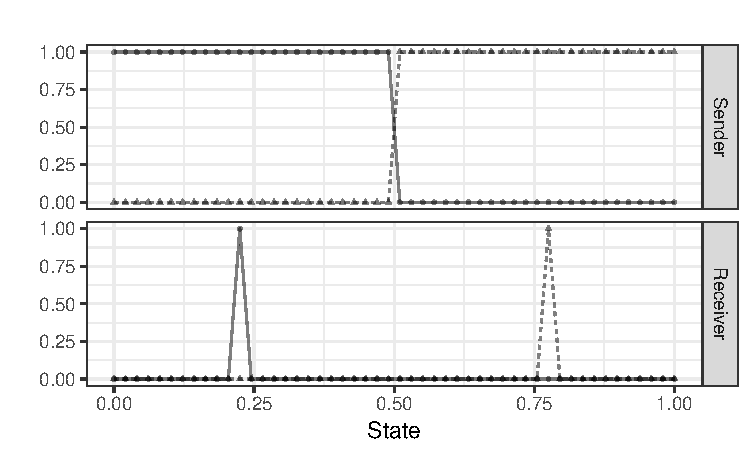
\includegraphics[width=\textwidth]{Rplot-example-strict.pdf}
    \caption{Crisp}
    \label{fig:example_stratsA}
  \end{subfigure}
  \hfill
  \begin{subfigure}[]{0.45\textwidth}
    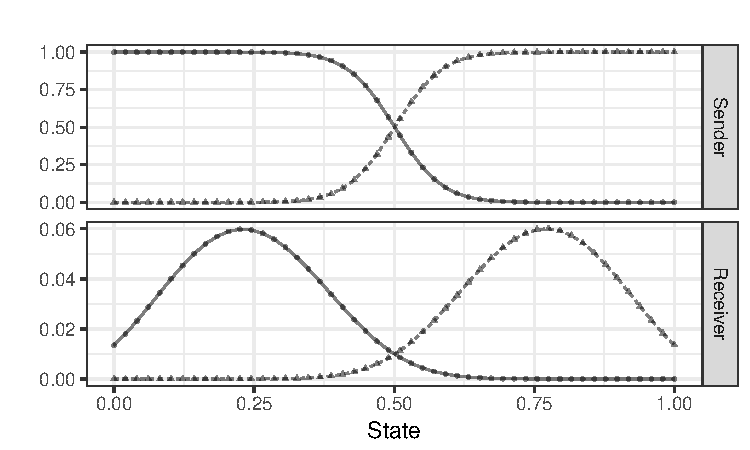
\includegraphics[width=\textwidth]{Rplot-example-vague.pdf}
    \caption{Vague}
    \label{fig:example_stratsB}
  \end{subfigure}

  \caption{Example strategies for a state space with 50 states. Each line corresponds to a message. For the sender, it plots for each state the probability that the message is used. For the receiver, it plots for each state the probability that the response is that state, given the message.}
  \label{fig:example_strats}
\end{figure}

In an abstract setup, using 50 states uniformly distributed over the unit interval and two possible messages, such an optimal language looks like what we see in Figure~\ref{fig:example_stratsA}.
The sender/receiver strategy pairs that we are looking for look more like Figure~\ref{fig:example_stratsB}.
While in the former the probability that the sender uses one message decays sharply from 1 to 0, and increases sharply from 0 to 1 for the other message, at a given point, in the latter these transitions are smooth.
This means that, for some states in the middle of the state space, there is uncertainty as to which message will be used, whereas for states in the extremes this is almost certain.
Similarly for the receiver strategy, in the first example for each message there is an almost certain response, whereas in the second example this is a degree of uncertainty.

The interpretation of this uncertainty will be different depending on the interpretation of the model.
If we see it as an explanatory model of how two agents play the game, we can see it as randomization.
If we interpret the model as descriptive, it simply represents expected behavior in a manner agnostic to the underlying mechanisms.
A third option is to see probabilities as capturing relative numbers in a population of agents.
For example, if the sender strategy assigns a probability of $0.4$ of message $m$ being sent for state $t$, this would mean that $40\%$ of the population uses that message for that state, while $60\%$ uses the other.
This latter option leaves open the possible interpretation that each agent commands a crisp language and vagueness is only a population-level effect.
However, given the level of abstraction of the description so far, none of this is necessarily implied by the model.
Our question is thus what additional modifications to sim-max games are sufficient for the optimal languages to be more like Figure~\ref{fig:example_stratsB}, rather than like Figure~\ref{fig:example_stratsA}.
%Let's look at some proposals in the literature.

% \subsection{Bounded rationality}
\textcite{franke_vagueness_2011} make two suggestions of how vagueness in a signaling game can arise as a consequence of limitations in the cognitive capacities of rational agents.
The first proposal is called limited memory fictitious play (LMF) and models agents playing a sim-max game where their ability to recall past interactions with others is limited to a certain number.
For a given interaction, each agent uses his limited memory of the other agent's past behavior to estimate the other's strategy.
Agents are assumed to be rational, thus each plays a best response (given the utility function) to their estimate of the other's strategy.
In order to observe the evolution of strategies in repeated interaction, this approach involves modeling several individual agents in actual play.
What the authors observe is the emergence of vague signaling at the level of the population, \emph{i.e.}~population averages of individual strategies exhibit the characteristics of a vague language as characterized before.
However, each agent still commands a crisp language, which is inadequate if the intention is to capture how vagueness presents itself in human languages.

In order to overcome this limitation, they make another proposal using the notion of a quantal response equilibrium (QRE).
The idea, inspired by experimental psychology, is to model the choice of best response as stochastic rather than deterministic.\footnote{Probabilistic choice rules are also the source of vagueness in recent accounts by \textcite{LassiterGoodman2015:Adjectival-vagu} and \textcite{QingFranke2014:Gradable-Adject}.} 
A prominent explanation for such soft-max or quantal choice behavior is that agents make small mistakes in the calculation of their expected utilities \parencite{Train2009:Discrete-Choice}. 
They still choose rationally the option with the highest expected utility, but each assessment of the expected utilities is noise perturbed.
This, in turn, may actually be optimal behavior if the calculation of expected utilities relies on assessing stochastic uncertainty. 
Choice based on a few samples from a distribution can be optimal if taking more samples or other means of better approximating degrees of uncertainty is resource costly \parencite[\emph{e.g.}][]{VulGoodman2014:One-and-Done-Op,SanbornChater2016:Bayesian-Brains}.
The degree to which agents tremble in the calculation of expected utilities and therefore deviate from the optimal behavior can be characterized by a parameter.
\textcite{franke_vagueness_2011} find that for low values of this parameter, only babbling equilibria (where sender and receiver simply randomize, respectively, message and response uniformly) where no communication actually occurs.
Above a certain value of the parameter, other equilibria of the kind described in the beginning of this section arise, where agents communicate successfully, though not perfectly, using fuzzy strategies similar to the ones depicted in Figure~\ref{fig:example_stratsB}. However, it is not clear that soft-max choices model the right stochastic trembles in decision making as they would arise under natural sources of uncertainty about the context \parencite[see][]{franke_vagueness_2017}.

% \subsection{Generalized reinforcement learning}
Cailin O'Connor~\parencite*{oconnor_evolution_2014} proposes a way in which vagueness could be expected to evolve as a side-effect of a particular type of learning process.
She studies sim-max games driven not by rational choice dynamics, but by generalized reinforcement learning (GRL), a variant of Herrnstein reinforcement learning (HRL)~\parencite{roth_learning_1995}.
In HRL, agents learn to play a signaling game by strengthening particular choices (of messages for the sender, of responses for the receiver) proportionally to how successful that choice proves to be in an interaction.
O'Connor's proposal is to model generalization as the propagation of reinforcement to nearby states, where ``nearby'' is defined in terms of distance in state space.
For example, if a sender was successful in using message $m$ for state $t$, he will not only positively reinforce that choice of message for $t$, but also for states similar to $t$.
This is done in a degree that is proportional to the degree of similarity between $t$ and other states.
The dynamics also gives rise to vague signaling of the kind we are looking for.

But why should agents evolve to generalize?
%First, it is not argued that vagueness in itself is beneficial, but that it is a by-product of a learning mechanism.
O'Connor suggests that, despite a vague language having lower expected utility than a precise one, the learning mechanism that induces vagueness does have evolutionary advantages, though not obvious ones (see \textcite{oconnor_evolving_2015} for the detailed argument).
Considerations of optimality of strategies are typically made in terms of hypothetical atemporal comparisons of expected utility.
However, generalized reinforcement learning has an interesting property in comparison with more strict learning mechanisms: it achieves higher payoffs in a smaller period of time.
In a naturalized evolutionary setting this temporary advantage should also be taken into account.
Imagine an initial population of agents with random strategies, some using GRL and others using classical Herrnstein reinforcement learning to adapt to each other.
Although the latter type of agent can hypothetically develop a precise and more efficient signaling system, agents using GRL would coordinate on vague signaling strategies with high (though not optimal) expected utility sooner than agents using HRL.
In such a scenario, they could drive the other agents to extinction before the latter had time to achieve coordination and reap the benefits of a more precise signaling system.

But would such a language be stable?
In terms of evolutionary game theory, one could argue that a small enough group of mutants playing a precise signaling system could later invade a population of vague signalers.
There is, an additional advantage to the generalized learning that is relevant here, namely the ability to adapt to a changing environment.
Analysis of a game in terms of evolutionary stable states works well if we assume that the environment where the agents interact remains static.
However, in a more realistic setting this is not the case.
In a dynamic game with a variable environment, an ability to converge faster could give an evolutionary advantage over strict learning rules: as soon as the state space or the utiliry function change, GRL would quickly adapt and again potentially drive more strict learning mechanisms to extinction because of their short-term gains.


% \subsection{Noisy perception}
\textcite{franke_vagueness_2017} study a variant of the replicator dynamics that is motivated by perceptual limitations.
Assuming that agents do not have perfect perception, there will always be a possibility that senders confuse states and receivers mix up responses.
Furthermore, it seems reasonable to assume that this state confusability is proportional to state similarity, \emph{i.e.}~that the more similar two states are, the more likely it is they will be mistaken for each other.
Incorporating thiese considerations into a derivation of the replicator dynamics based on imitation processes, they develop a variant of that dynamic that also induces vague signal use of the kind we expect here.
The consequence is very similar to that of the GRL model discussed above, in that the way the behavior for a given state is updated takes into account the behavior of similar states, proportionally to their similarity.
Given the known relation between reinforcement learning and the replicator dynamics~\parencite{Beggs2005}, it is actually quite plausible that the two are tightly related, but this would need to be formally demonstrated.
The account is, however, interpretable at a lower level of rationality since the replicator equation is suitable to represent biological processes of natural selection.

The motivation underlying this model of vague signaling is still one of inevitability.
A vague strategy is still not claimed to have higher expected utility than a crisp one.
However, the authors observe an effect similar to that pointed out by~\citeauthor{oconnor_evolution_2014}: signaling converges faster in scenarios where there is some degree of state confusability.
Furthermore, they observe one additional potentially beneficial property.
By running several rounds of simulation for each parameter set, they can measure how close resulting strategies are to each other within each group, and how they would fair playing against each other by calculating a within group expected utility.
The results show that the within group distances between strategies is smaller with growing confusability, and the within group expected utility is actually higher for strategies evolving under a certain degree of state confusion.
Thus, some amount of uncertainty seems to promote more homogeneous populations of signalers that are better at achieving cooperation within a group of such signalers

% \subsection{Aggregation from multiple senders}
\textcite{lawry_vagueness_2017} explore the potential benefits of vagueness in variations of a sim-max game with multiple senders and one receiver.
Although the models considered are not explicitly identified as sim-max games, they are equivalent in the relevant aspects: they are signaling games where senders have private knowledge of a given state $x$, each sends a message to the receiver, which then selects an estimate $y$ of the original state; although the authors do not define a utility function, their analysis evaluates the models in terms of the expected error between the estimate and the original state, defined as $(x-y)^2$; better models have lower expected error, thus one could say that the objective is to minimize this function, which would be equivalent to maximizing its inverse; the game could then be seen as a sim-max game with multiple senders and negative squared difference as similarity function.
Unlike the models discussed so far that introduce minimal constraints to a dynamic and study the strategies that emerge out of an evolutionary process, these authors' approach is mostly static and analytical.
They consider several possible sender strategies with uncertainty and without and calculate if and when sender and receiver achieve better transmission accuracy, \emph{i.e.}~smaller expected error between original state and receiver estimate.
Senders without uncertainty have a strategy that boils down to what is represented in Figure~\ref{fig:example_stratsA}: they split the state space according to a fixed thresholds, switching from using one message to another abruptly.
The model for the other type of sender is similar, but assumes that there is uncertainty regarding the value of the thresholds, representing them as uniformly distributed random variables.
What results from this in terms of sender strategy is also a smooth transition between the use of two messages, but unlike what we see in Figure~\ref{fig:example_stratsB}, it is a linear transition\footnote{This is certainly connected with the choice of modeling the uncertain threshold as uniformly distributed. We speculate that another choice of distribution, like for example a normal distribution, would yield something similar. What is important to characterize a vague use of messages, however, is that the transition is smooth and monotonous, not its particular shape.}.
The receiver strategy is not inherently vague for either type of sender, it merely aggregates the messages received to provide an estimate of the original state using a simple arithmetic mean.

The authors analyze a number of variations of this model.
For a model with one sender, results are consistent with Lipman's~\parencite{lipman_why_2009} in that strategies without uncertainty lead to more accurate communication.
For models with two messages and more than one sender, the expected error is a strictly decreasing function of the number of senders, and above a certain number of senders, strategies with uncertainty actually achieve lower expected error than sharp ones.
This minimal number of senders from which vagueness surpasses sharpness is a decreasing function of the number of messages, \emph{i.e.}~whereas at least 8 senders are needed if the number of messages available is 2, this number lowers to 5 for 3 messages, 4 for and 5 messages, and 3 for more than 6 messages.
If random errors are introduced between the choice of the sender and the message that reaches the receiver, increasing the number of senders can compensate for the noise, to a certain extent.
Results are mixed when dropping the assumption of uniform priors for the state space.

These results are interesting since they reveal scenarios where vague strategies have an advantage over strict ones, even in a setting of higher rationality.
The approaches discussed so far argue that vagueness is the inevitable byproduct of either cognitive limitations or a particular learning mechanism in the context of other learning mechanisms, which still leaves the idealist\footnote{In an ordinary, non-philosophical, sense.} some room for speculation.
In the models of \citeauthor{franke_vagueness_2011}, the idealist could argue that higher rationality (or better memory) would lead to more precision.
\citeauthor{oconnor_evolving_2015}'s learning strategy could theoretically be dominated by a process with higher strategic rationality, like best response dynamics~\parencite{ellison_learning_1993}\todo{is this the canonical reference?}.
A combination of both would hypothetically lead to a better outcome in the scenario of \citeauthor{franke_vagueness_2017}.
However, \citeauthor{lawry_vagueness_2017} give us something that holds even if the idealist is unwilling to acknowledge the constraints that permeate our finite existence.
Whether the scenario of multiple senders is representative of the language games where vagueness comes about, and whether the strategies proposed by the authors would be the ones to evolve\footnote{Their analysis is a static one. Despite the advantage of the proposed vague strategies against strict ones in certain settings, one cannot know whether other strategies of higher accuracy would not be possible in those same settings without studying some dynamics in an evolutionary context.}, is something that is, however, open for debate.


\section{Vagueness in multiple reference games}
\label{sec:referential-vagueness}

Linguistic interaction, as captured by a sim-max game, has a rather narrow scope. There is a fixed prior, a fixed utility function and a fixed similarity measure between states. 
If the sender observes a state $t$ and the receiver guesses state $t'$ the utility of that interaction is proportional to the similarity between $t$ and $t$. 
Here is a natural example of a situation captured by a sim-max model: Kiki wants Bubu to draw her dissertation cover in a particular shade of blue $t$; the closer Bubu's color choice matches Kiki's idea, the better. Here Kiki wants to \emph{describe} the color for Bubu to pick out or realize from the whole set of possibilities. 
It's a natural thing to want to do with language. 
But a lot of communication with vague and contiguously variable properties is rather different. 
In the general spirit of Wittgenstein's method of arranging multiple language games side by side for a more encompassing picture, we should look at some more cases of language use as well. 
Let us therefore consider a continuum of cases of referential communication.

A \emph{reference game} is a model of a situation in which the speaker has a particular object in mind and uses a description in order for the receiver to pick this object and no other object. 
One crucial difference to descriptive communication and sim-max games is that close will not be close enough: if Kiki needs a long nail, a nail a little longer or shorter may be good enough; but if Bubu needs the long, slightly bend nail with the flat top (which she previously disassembled from her art installation), no other nail will do. 

Interestingly, referential communication can take place under a plethora of different epistemic conditions. 
A lot of modeling work considers \emph{reference games without displacement} where sender and receiver communicate about a context, i.e. a set of objects, which is immediately accessible in their direct perceptual environment \parencite[\emph{e.g.}][]{BaronchelliGong2010:Modeling-the-Em,Franke2012:Scales-Salience,Franke2012:On-Scales-Salie}.
Agents may make mistakes about observing exactly how blue or long etc.~a particular object is, but there is no further fundamental uncertainty about the context. 
This, of course, need not be so. \textcite{lipman_why_2009} and \textcite{Deemter2009:Utility-and-Lan}, for example, consider \emph{reference games with displacement}. 
Kiki asks Bubu to fetch the red book from the library. 
No other book than the one Kiki needs will serve. 
When Kiki describes the book, the perceptual context in which Bubu must make her choice is not co-present to Kiki at the time of speaking. 
Yet other situations are imaginable. 
In \emph{reference games with partial uncertainty}, for instance, interlocutors may know that they have shared and immediate access only to a subset of the objects in the context, but be uncertain about whether the co-player sees any other objects. 
This is the set-up for the classic director task in psycholinguistics \parencite[\emph{e.g.}][]{KraussGlucksberg1977:Social-and-nons,Keysar2000,KeyzarLin2003:Limits-on-Theor}.

What would a rational agent do in repeated reference games? 
Take a universe in which agents play repeated reference games without displacement. 
A single game has sender and receiver both flawlessly perceive a context of $k$ objects (with $k$ possibly randomly drawn for each encounter); each object has its individual features, e.g., drawn from a rich multidimensional feature space of continuously variable properties \parencite[\emph{e.g.}][]{Franke2012:Scales-Salience,Franke2012:On-Scales-Salie}. 
The sender chooses a message $m$ for the target object $t$, but she can condition her choice on the current context $c$. 
Likewise, the receiver chooses a referent $t'$ from the available objects in $c$, again conditional on $c$. 
But if agents play many such reference games with different contexts $c$ and $c'$, and if strategic rationality means to signal and interpret so as to coordinate on the correct referent, strategic rationality of local choices in $c$ and $c'$ is not enough to guarantee that agents' beliefs and behavior in $c$ have any relation to their beliefs and behavior in $c'$. 
An agent could use a certain signal to denote, say, the tallest object in every context with between five and twelve objects or when the number of objects is a prime number, but use the same signal for the darkest object in all other contexts.
This could even be rational if most agents do it this way.
It could evolve as a convention under selection for communicative success as well.
In other words, neither local strategic rationality in a fixed context nor evolutionary adaptation to each single context entails a natural, globally consistent behavior across multiple contexts. 
The situation only gets worse if we want to have agents use the same expressions in a consistent way also across different types of reference games, with possibly different epistemic conditions. 

The picture sketched in the last paragraph neglects learning from observation and generalization across contexts. 
For rationality, we need to consider a rational agent's ability to learn from previous experience and to generalize from  the past to the future. 
For evolutionary adaptation, the story so far misses the key fact that languages and practices have to be learnable in appropriate time from the actual observables, lest what is learned and further transmitted will simply be a different language or practice \parencite[\emph{e.g.}][]{KirbyGriffith2014:Iterated-Learni}.
But even if every language learner in history had been perfectly rational, it is extremely unlikely that anyone ever succeeded in reducing all uncertainty about language use and say with confidence: this is the threshold that truly separates heaps from non-heaps no matter what. 
For one, there may simply not be enough time in the lifespan of a rational learner to observe enough instances of language use for certainty about crisp denotations. 
For another, what needs to be learned likely changes over time. 
The optimal use for gradable properties hinges crucially on the prior over states \parencite[\emph{e.g.}][]{Franke2012:Scales-Salience,Franke2012:On-Scales-Salie,QingFranke2014:Gradable-Adject,LassiterGoodman2015:Adjectival-vagu}. 
If the prior captures real world attributes, such as the probability of an individual's body height, these attributes will not only be hard to know for certain, but they will also vary over time. 
They may also depend on location: do we use our language exclusively in this village or do we travel beyond? 
If so, the priors that determine the goodness of a convention for one agent need not be the same as those for another. 
Going beyond the priors for property degrees, the probability of seeing a particular language game, e.g.~a particular context $c$ in some kind of reference game, is also crucial for determining globally efficient linguistic behavior. 
But here it is even more inconceivable how a rational learner could acquire a fairly confident estimate over how often a particular language game will be played. 
The list of sources of natural and seemingly insurmountable uncertainty about the parameters necessary to determine locally or globally optimal strategies is much longer than hinted at here. 
Still, it should be clear enough that a finite existence, a sparse learning input and the inherent fuzziness of the linguistic context itself (its temporal, local and social variability) is not a faul of rationality or the mechanism of selection of successful linguistic practices. 

What about meaning and vagueness in a universe of multiple language games and heavy uncertainty? 
We could look for meaning at several levels. 
Firstly, as before, there is the actual behavior of a single agent in each actualized language game. 
As mentioned above, behavior that strictly maximizes expected utility under uncertainty may be resource heavy, so it might be compatible with local strategic rationality that agents' production choices are stochastic (with the caveat that in the real world we would never know because we cannot ever elicit a production in the exact same circumstances in a constantly changing environment including the mind of a speaker).
Secondly, if we look at behavior across many game types and contexts, there is also the level of an agent's internal theory of how words and phrases are likely to be used, conditional on a given context. 
Notice that a single agent's rational beliefs about linguistic practices or linguistics meaning may well have to reflect the actual stochasticity: under natural assumptions about information loss, the best belief for prediction matches the actual distribution in the real world \parencite[\emph{e.g.}][]{VehtariOjanen2012:A-survey-of-Bay}.
Either one of these two levels, the agent's behavior or linguistic generalizations, could be the foundation for a notion of emerging abstract meaning as constituted by the practices of a population at a particular time.
If both agents' rational behavior and rational beliefs are plausibly fuzzy, why should a concept of supervening meaning be crisp? 
Maybe there is a reason.
The main question to be answered is even more general: given a universe of (rational) language users who learn from finite experience in a changing and stochastically complex arrangement of multiple language games, is a notion of linguistic meaning a theoretically useful and empirically explanatory concept in this picture in such a way that if that notion entailed vague meanings the whole view would have disastrously little explanatory bite?

Taken together, when we look at the picture of multiple language games side by side, the question of what rational or optimal behavior is in any one of them, or the question of why human language users do not more closely approximate rational or optimal local behavior more closely seem entirely misplaced.
What seems more pressing is to answer how the interaction of individual learning, individual local optimization and general pressure for successful communication at a cross-situational level lead to the shaping of linguistic practices in an open-ended landscape of language games.
How to attain locally sub-optimal play in a single language game is not a theoretical puzzle we should take serious, if what really matters is a global multi-game perspective.
Adopting this perspective does not \emph{solve} the problem of how vagueness is compatible with rationality. 
But it suggest that it might be an inflated issue that we need not or should not worry about, because it will not matter for a more general and pressing issue in a more realistic and encompassing picture of language, its use and evolution. The following section will expand on this.




% \section{Vagueness in related models}
% \label{sec:other-vagueness}
%
% \subsection{Preference misalignment}
% \todo[inline]{Test CS~\parencite{crawford_strategic_1982} results in our model by using bias in utility function. READ Förster, M., and Riedel, F. (2011). Distorted Voronoi languages (working Paper). -> distorted Voronoi languages, i.e. shifted according to bias, but still crisp}
%
% \subsection{Noisy communication}
% \todo[inline]{Test if noise in communication channel as modeled by Blume~\parencite{blume_intentional_2014} induces vague strategies as well}


\section{How could language not be vague?}
\label{sec:finite-experience}
Arguments of the kind presented by Lipman~\parencite*{lipman_why_2009}, that a vague language is suboptimal compared to a crisp one, work under a number of various assumptions.
Together, they form a picture of the context where agents learn and use language that is highly idealized.
This picture has been criticized for several decades, at least in the field of theoretical economics.
Herbert A.~Simon describes it as such:
\begin{quote}
Traditional economic theory postulates an ``economic man,'' who, in the course of being ``economic'' is also ``rational.''
This man is assumed to have knowledge of the relevant aspects of his environment which, if not absolutely complete, is at least impressively clear and voluminous.
He is assumed also to have a well-organized and stable system of preferences, and a skill in computation that enables him to calculate, for the alternative courses of action that are available to him, which of these will permit him to reach the highest attainable point on his preference scale.%
~\parencite[99]{simon_behavioral_1955}
\end{quote}
Perhaps this could be seen as the setup of a straw man argument, but we believe it captures some of the crucial assumptions that still underlie some game theoretic models of language.

In fact, in order to account for vagueness in natural language in the context of these models, the proposals surveyed here all need to peel away from this idealized model of agents, language, and the world, and bring some of these assumptions down to earth.
They suggest various mechanisms that can lead to vague use of messages in certain signaling games, such as cognitive limitations like a finite memory or the inability to always calculate the absolute optimum choice to make, learning mechanisms that compensate for the finiteness of experience through generalization based on similarity, imperfect senses that allow for the possibility of stimulae to be confused, etc\todo{fit Lawry and James plus referential games stuff}.
In the process, we realize ways in which we, as language learners and language users, are finite beings finding ways to cope with a highly complex and dynamic world:
\begin{enumerate}
\item Our existence is temporally finite; language does not have an infinite amount of time to evolve or take a long time to be learned. The faster a language can start to be useful, the better;
\item Language learning through experience has to rely on a limited number of observations. Not only is the state space typically much larger than what one can survey in sufficient time, but it is also potentially infinite and constantly changing;
\item A corollary of the former is that there will always be heterogeneity in a population of language learners, at least of prior experience since each agent will have relied on a different set of observations. Furthermore, this information is not directly or fully accessible to others;
\item Given that an agent is almost always learning and using language in such a population of other agents, there are also various potential sources of linguistic input the agent is constantly integrating in his practice;
\item We do not play only one language game in our existence; there is a plurality of them and which one an agent is engaged in at a particular moment is never clearly identified, neither are the exact benefits one might take out of it by choosing a certain behavior over another;
\item These are furthermore not fixed in time; old language games fall out of fashion or stop being useful, and new ones emerge all the time.
\end{enumerate}
All of these observations support the weakening of our modeling assumptions.
% If we take these points seriously, we have to concede that it is almost inevitable that uncertainty gets introduced at almost all levels of language learning and language use.
% In the context of a signaling game, we can expect uncertainty about priors, observations, utilities, behavior of other players, and more.
% This is true both from the perspective of the modeler, as from the perspective of the agents involved, supporting the motivation to take it into account in our modeling efforts.

The research surveyed here shows us some examples of assumptions which, when weakened, make vague signal use a natural outcome of certain evolutionary dynamics.
But it gives us even more.
We learned from \citeauthor{oconnor_evolution_2014} and \citeauthor{franke_vagueness_2017} that vague languages are quicker to converge and more adaptable, which is valuable given the finite and dynamic character of our experience (point 1).
\citeauthor{oconnor_evolving_2015} also showed how generalization, an invaluable feature of any procedure for learning from a limited number of observations (point 2), leads to vagueness.
We also learned from \citeauthor{franke_vagueness_2017} that state confusability, a mechanism thats leads to vague signal use, can have a homogenizing effect on vocabularies, potentially compensating for the heterogeneity of agents' experiences (point 3).
\citeauthor{lawry_vagueness_2017} demonstrated the benefits of strategies that incorporate uncertainty, leading to vagueness, in language games where agents need to aggregate information from various sources (point 4).
\todo[inline]{add something for 5 and 6, maybe referential games}
%Trying to answer the question of ``Why is language vague?'', is important to force us to recognize those aspects of language and the world that are easily forgotten when idealizing the subject matter.
%The finiteness of human experience, the dynamic nature of the world, and the communitarian context of language use and development, these are things we need to keep in mind lest we end up with inadequate models of language and meaning.
% Wittgenstein put it better:
% \begin{quote}
% The more closely we examine actual language, the greater becomes the conflict between it and our requirement. (For the crystalline purity of logic was, of course, not something I had discovered: it was a requirement.) The conflict becomes intolerable; the requirement is now in danger of becoming vacuous. – We have got on to slippery ice where there is no friction, and so, in a certain sense, the conditions are ideal; but also, just because of that, we are unable to walk. We want to walk: so we need friction. Back to the rough ground!%
% ~\parencite*[\S 107]{wittgenstein_philosophical_1953}
% \end{quote}

What do these observations tell us about rationality?
% The replicator equation lends itself to an interpretation where agents could be said to be devoid of rationality, procedural or instrumental.
% This is the case where we see the equation as purely descriptive of a population of agents with hardwired behaviors, where the most successful strive and the least successful die off.
% In such an interpretation there is no room for questions regarding the rationality of vagueness.
% Another possible interpretation is that of a population of agents learning by imitation.
The LMF dynamics of~\textcite{franke_vagueness_2011}, generalized reinforcement learning~\parencite{oconnor_evolution_2014}, and the work of~\textcite{franke_vagueness_2017}, all paint a picture of agents with a basic level of instrumental rationality, very limited awareness of the game, and a lack of strategic capabilities, adapting their behavior with only short-term gains in sight.
Under the standard assumptions, even agents with such limited rationality would evolve crisp signaling in sim-max games.
All approaches introduce constraints into the dynamics that prevent the evolution of crisp signal use.
But a crisp language would still have a higher expected utility than the evolved strategies.
Agents in those models seem to be rational only to the extent of their capabilities.
Despite the plausibility of the mechanisms proposed (limited memory, generalization, state confusability), this feels like a bittersweet conclusion because of this hypothetical possibility of a better, hence more rational, strategy, that seems to be only artificially barred from the agents.
But this is so only if rationality is equated with maximization of expected utility.
The mechanisms that lead to vague signal use, as~\textcite{oconnor_evolution_2014} and~\textcite{franke_vagueness_2017} stress, have the aforementioned important advantages of faster speed of convergence, higher flexibility, and homogenization.
These advantages matter, especially in the complex, dynamic context of real language use.
One would thus like to say that using a strategy that promotes those characteristics without a significant loss of expected utility is certainly a rational choice.
But in order to be able to say that in the context of the model, we need either a notion of rationality that goes beyond maximization of expected utility.

For more complex agents, the story is potentially more nuanced.
Consider an agent that has awareness that something like a game is being played, some estimate of the potential payoff involved, ability to gauge other players' expected behaviors, and the capacity to think strategically.
Is it rational for a sender to use a message in a crisp way, splitting the state space as if a strict threshold existed between the use of one term and the other?
In a scenario where the agent ability to make the optimal choice is bounded, such as the QRE model of~\textcite{franke_vagueness_2011}, the agent is again doing the best he can given the constraints imposed on him.
\textcite{lawry_vagueness_2017} draw attention to another option we need to consider: such agents could opt to ignore their limitations and external sources of uncertainty and use a crisp strategy regardless.
The authors' analysis shows that such an approach would be irrational in a number of different scenarios, even in the narrow interpretation of rationality as utility maximization.
But even in other scenarios, we could again argue that, if we broaden our notion of rationality, it would be less rational to use a crisp strategy rather than one that incorporates at least some source of uncertainty.
A crisp strategy for a particular game would, in most realistic scenarios, take more time to achieve convergence, be less adaptable to changes, less easy to reuse in other similar games, and less able to foster cooperation with a bigger group of agents.

Thus, if we pragmatically acknowledge the complex and dynamic environment that surrounds language learning and use, we find many plausible sources of uncertainty that can lead to vague signal use.
Furthermore, if we broaden our notion of rationality beyond mere maximization of expected utility, we also find reasons to welcome the positive aspects of these processes and to see their acceptance as a perfectly rational choice.
The investigation doesn't end here, though.
The research discussed here suggests that although vagueness can be beneficial, that is the case only in moderation: too much can lead to babbling equilibria where no information is transmitted.
Thus, for agents capable of adjusting the level of vagueness in their strategies, questions remain regarding how this can be modeled and what factors influence the amount of vagueness that is optimal for a given situation.
Other challenges include how to incorporate the intuitions about the relevance of the aspects enumerated above into our models.

\section{Conclusion}
\label{sec:conclusion}

\printbibliography

\end{document}
